\clearpage
\section{Data quality aspects and background validation}
\label{sec:data-quality}

During the run 2 data taking period of \gls{cms}, there have been a few detector issues that require some special care. Following the central recommendations, three issues are handled here, namely, L1 prefire rate in 2016 and 2017, \gls{ecal} Endcap (EE) noise in 2017, and the HE minus side (HEM) failure in 2018. In the process of dealing with these issues, the jetty background data-driven method is also validated in data. 

\subsection{L1 prefire issue in 2016 and 2017 data}

The L1 prefire issue in 2016 and 2017 happened due to an \gls{ecal} timing error, which was propagated to the L1 trigger primitives. This issue occurred because the trigger system used data from the previous bunch crossing rather than the current one to determine whether an event should be triggered. Events with significant ECAL energy in the region $2.5<\abs{\eta}<3$ are affected in 2016 and 2017 data. This can lead to inefficiency and was studied for signal Monte Carlo samples, as it can potentially lower the signal event count. Prefiring weights were added to signal and checked against the unweighted events, and no significant effect was observed. Data was also checked with and without the prefiring weights for the most affected period of 2017 by looking at closure plots in a same-charge \gls{cr}. This serves both to validate that the prefire issue does not affect this analysis and to act as a data validation for the jetty background. Plots can be seen in Section~\ref{sec:same-sign-validation-plots}.

\subsection{EE noise in 2017 data}

In 2017 data, an observed excess of fake \ptmiss compared to simulation was caused by increased noise in low-\pt jets. Additional noise in the \gls{ecal} endcaps in data was identified as the cause of this effect. To deal with this issue, the recommendation is to recalculate \ptmiss, excluding jets in the affected phase space. This was done centrally in the process of creating the samples used in this analysis.

\subsection{HEM failure in 2018 data}

Following the power interruptions generated by false fire alarms on Saturday, June 30th, negative endcap \gls{hcal} sectors HEM15 and HEM16 could no longer be operated until the end of the 2018 run. The affected $\eta-\phi$ region is $-3.0<\eta<-1.3$ and $-1.57<\phi<-0.87$. The first regular physics run affected is 319077. Data and simulation vetoes for objects in the affected region are applied. Same-sign validation plots are made pre-HEM and post-HEM in order to see their effects. The well-behaved validation plots suggest that this analysis is not badly affected by this issue.

\subsection{Same-sign validation plots}
\label{sec:same-sign-validation-plots}

Figure~\ref{fig:same-sign-validation-plots} shows data validation plots for the same-charge control region. They serve both as background method validation and to check the data taking issues mentioned above. The plots are divided into different data taking periods to check the effects of the data taking issues. The same-sign control region has been selected since it can validate the assumption that the isolation sideband properly predicts the shape of the main band and can therefore be used as the estimation method. Overall, good shape agreement is demonstrated between the main band and the isolation sideband.

\begin{figure}[!htb]
\centering
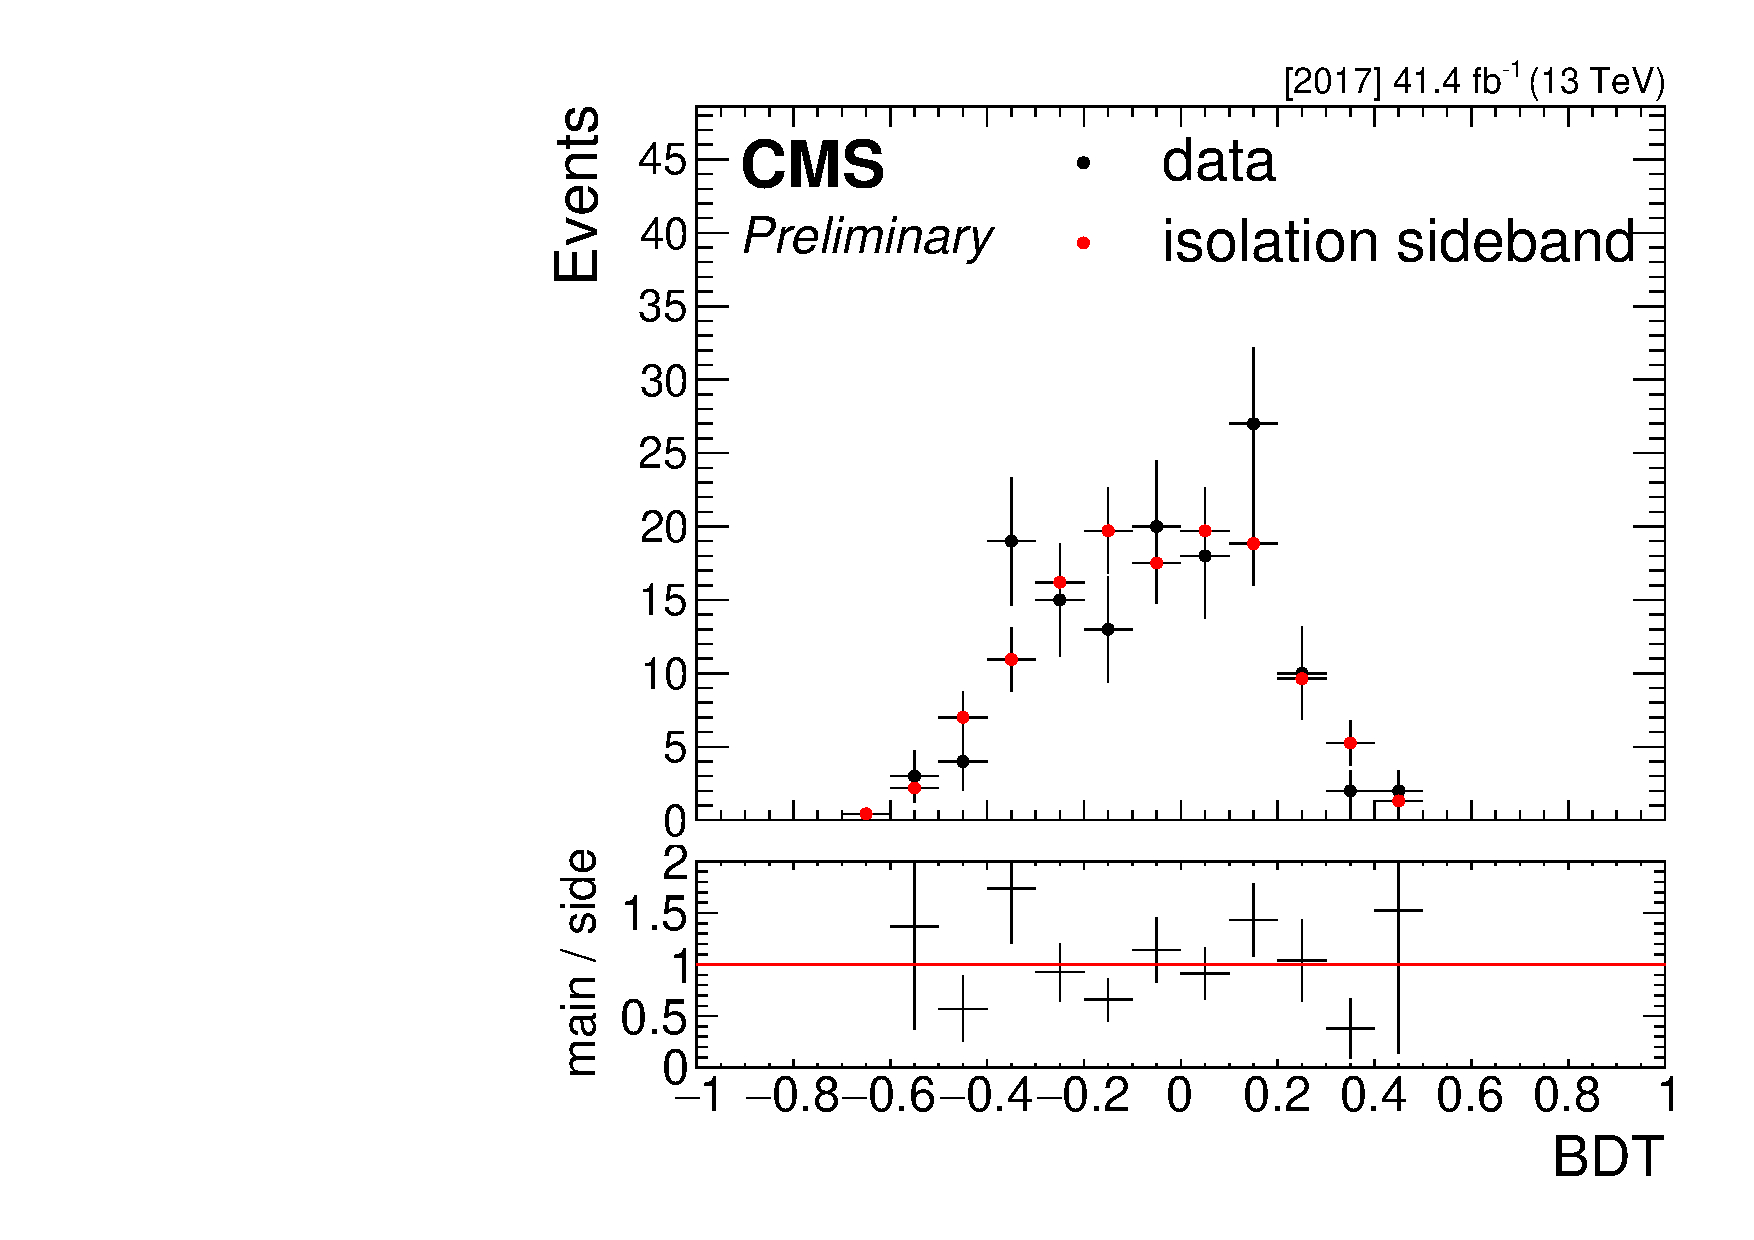
\includegraphics[width=0.48\linewidth]{plots/dilepton_muons_data_isocr_no_retag_CorrJetNoMultIso10_06_invmass_same_sign_2017/none_dilepBDTCorrJetNoMultIso10Dr0.6.pdf} \,
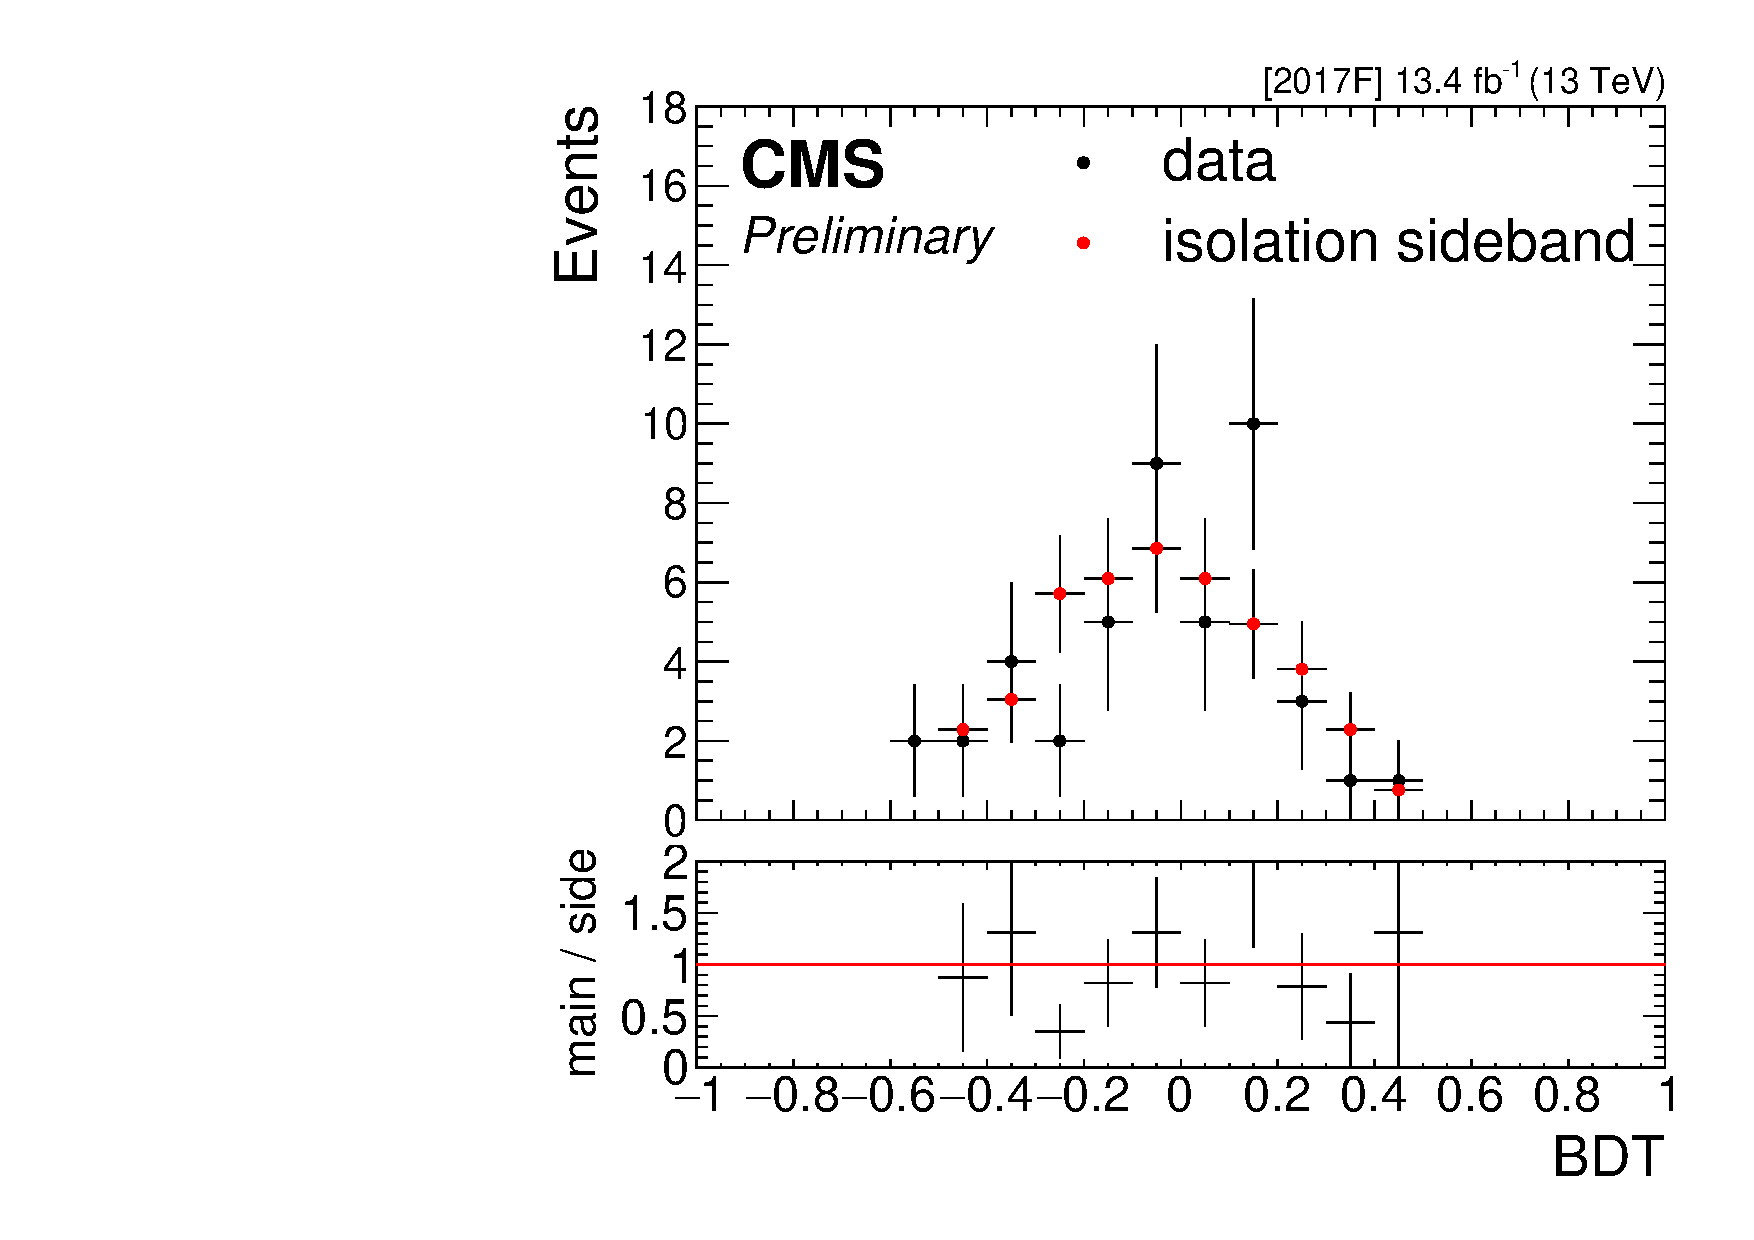
\includegraphics[width=0.48\linewidth]{plots/dilepton_muons_data_isocr_no_retag_CorrJetNoMultIso10_06_invmass_same_sign_2017F/none_dilepBDTCorrJetNoMultIso10Dr0.6.pdf} \\
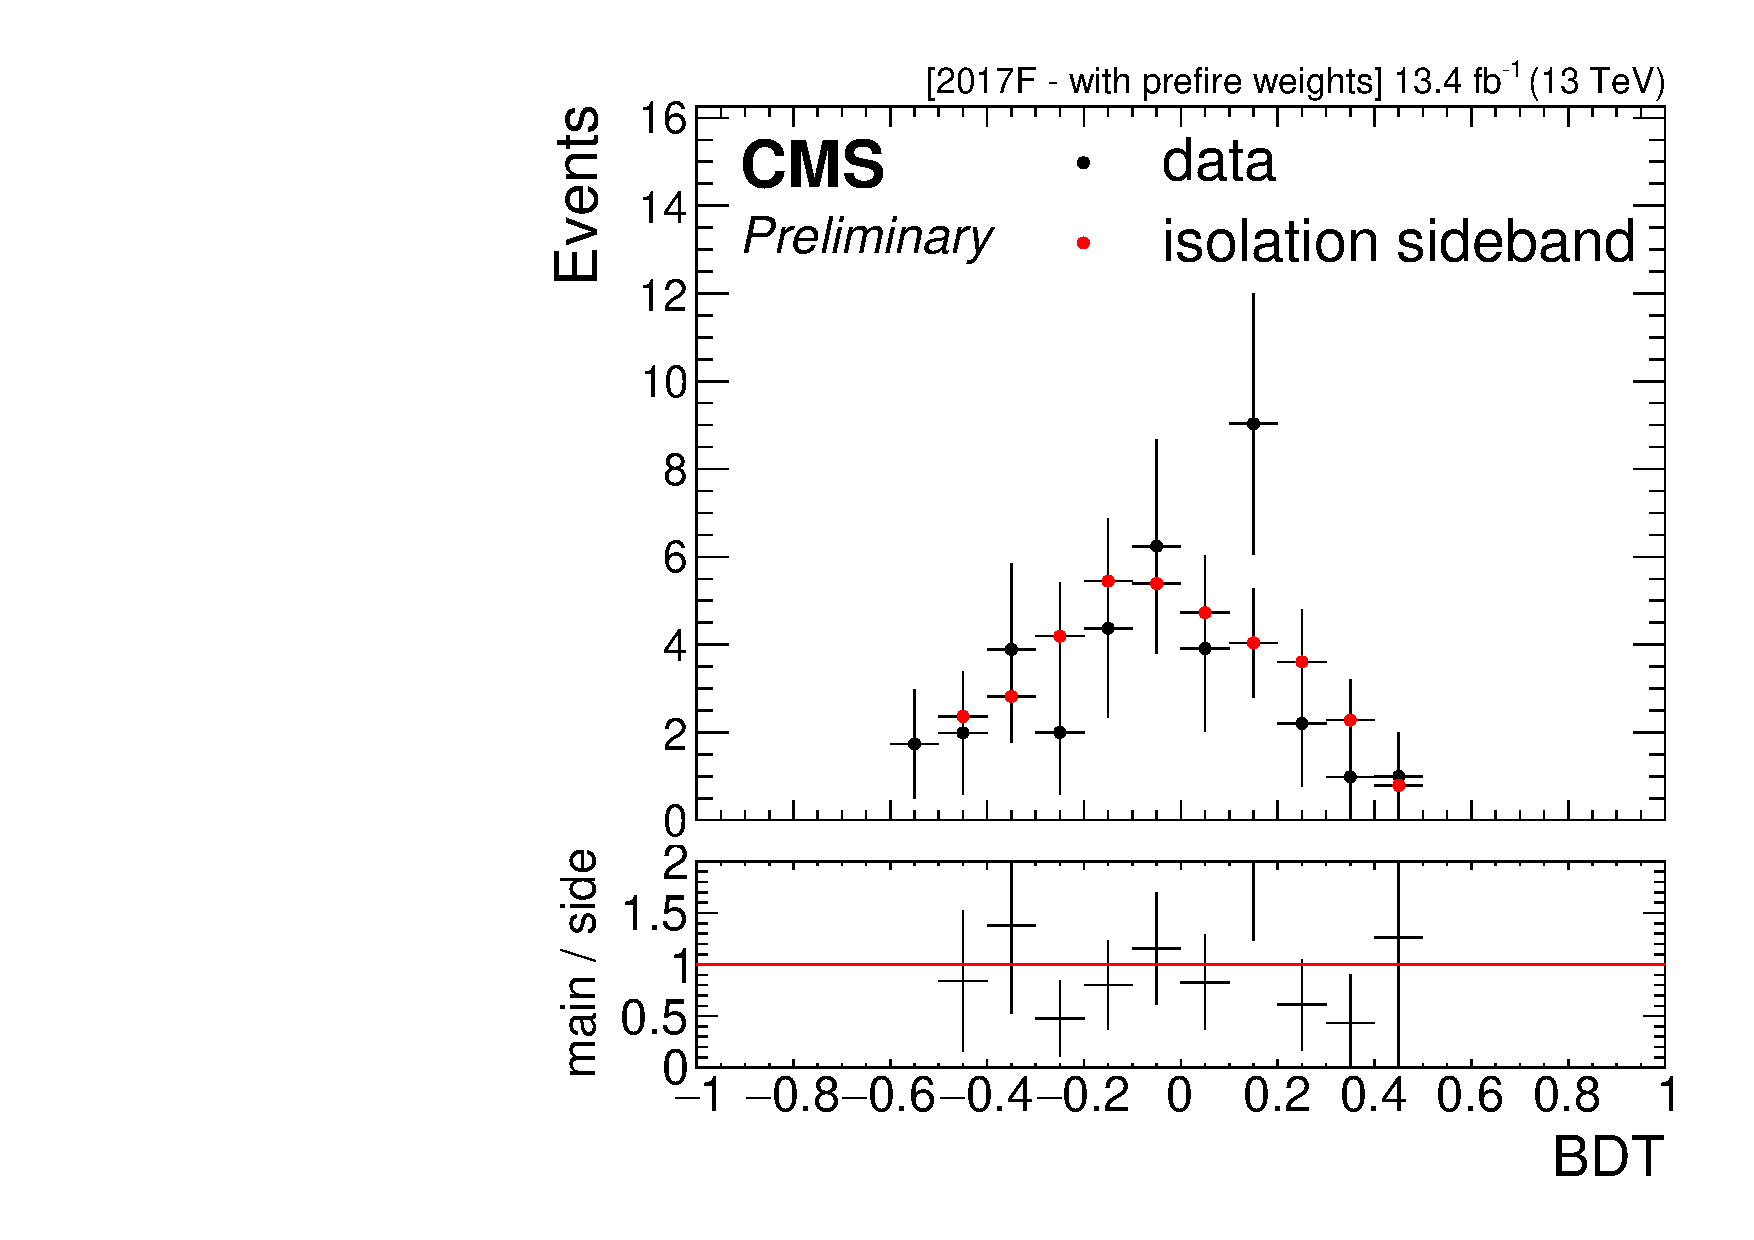
\includegraphics[width=0.48\linewidth]{plots/dilepton_muons_data_isocr_no_retag_CorrJetNoMultIso10_06_invmass_same_sign_2017F_prefire/none_dilepBDTCorrJetNoMultIso10Dr0.6.pdf}  \,
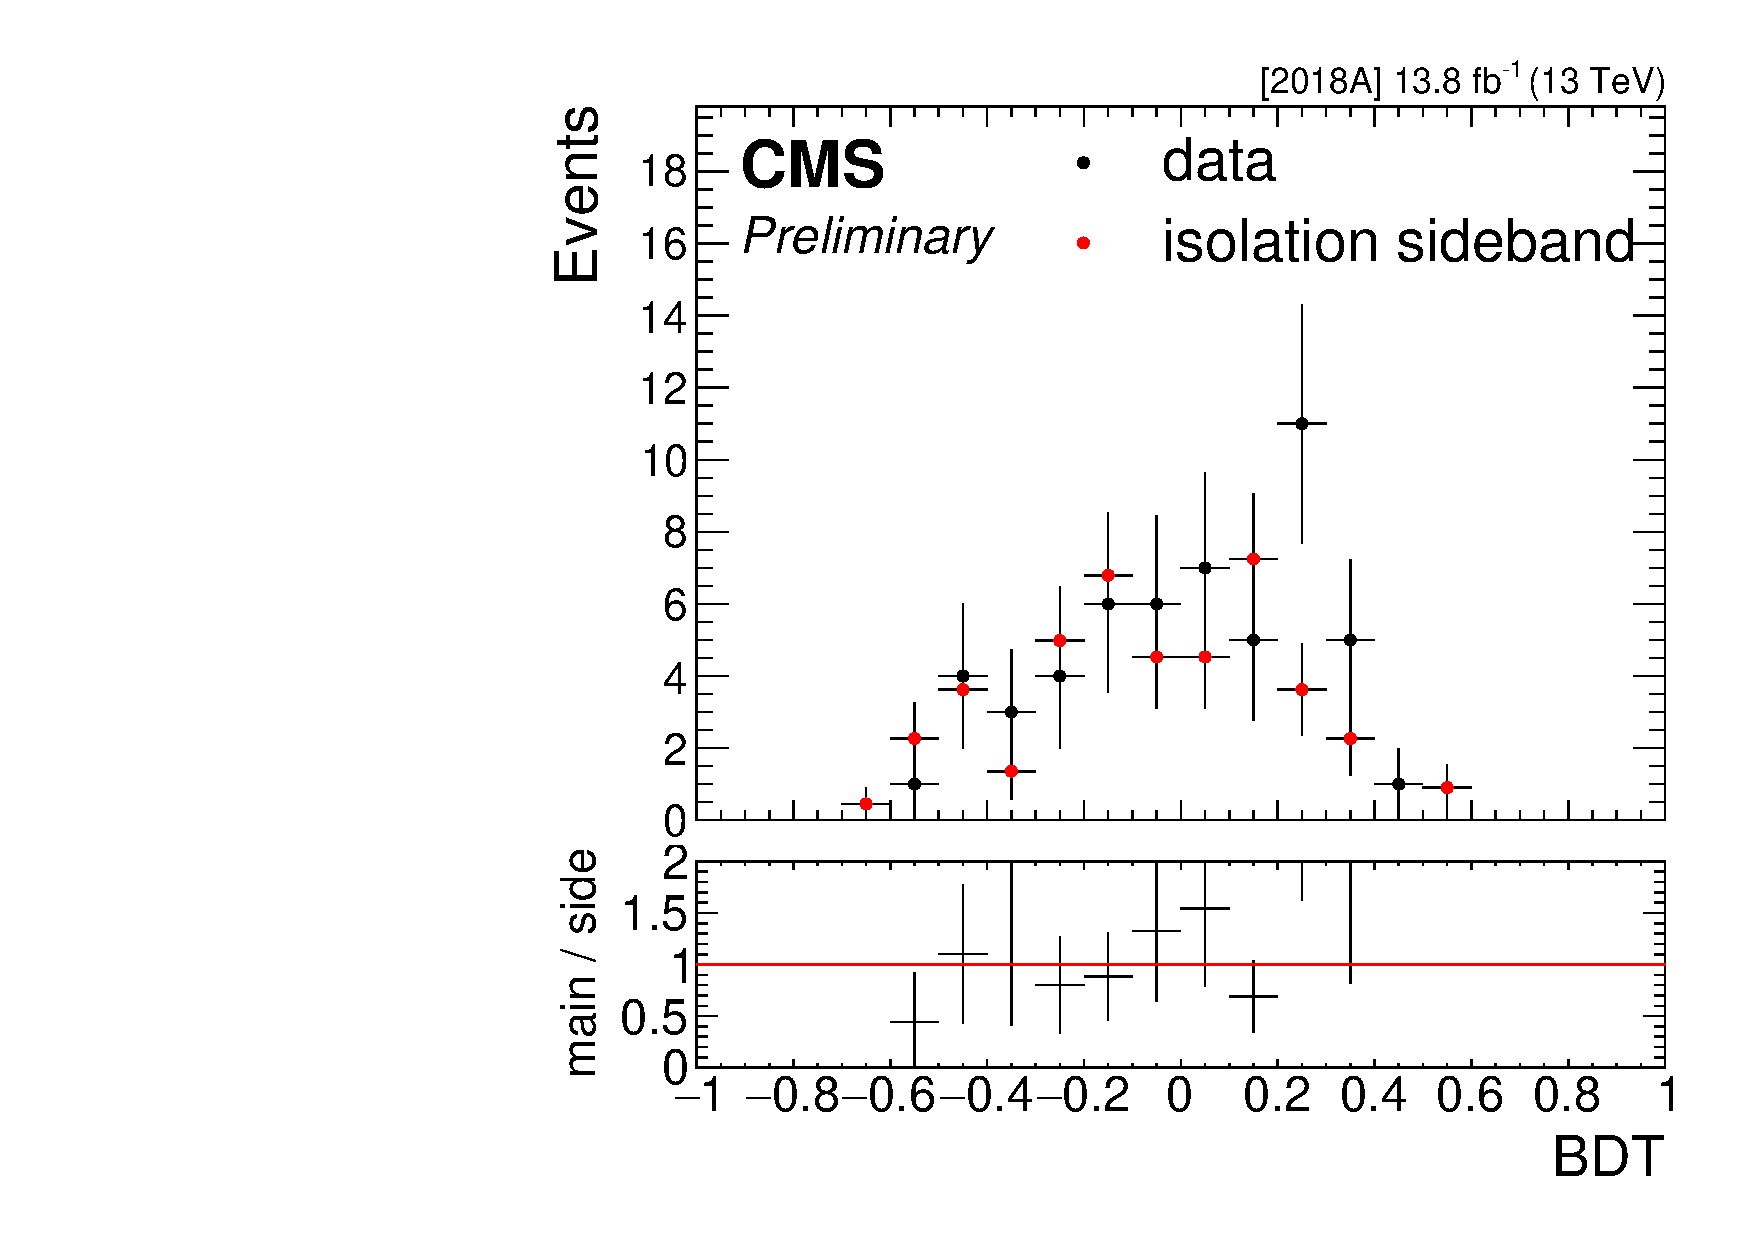
\includegraphics[width=0.48\linewidth]{plots/dilepton_muons_data_isocr_no_retag_CorrJetNoMultIso10_06_invmass_same_sign_2018A/none_dilepBDTCorrJetNoMultIso10Dr0.6.pdf} \\
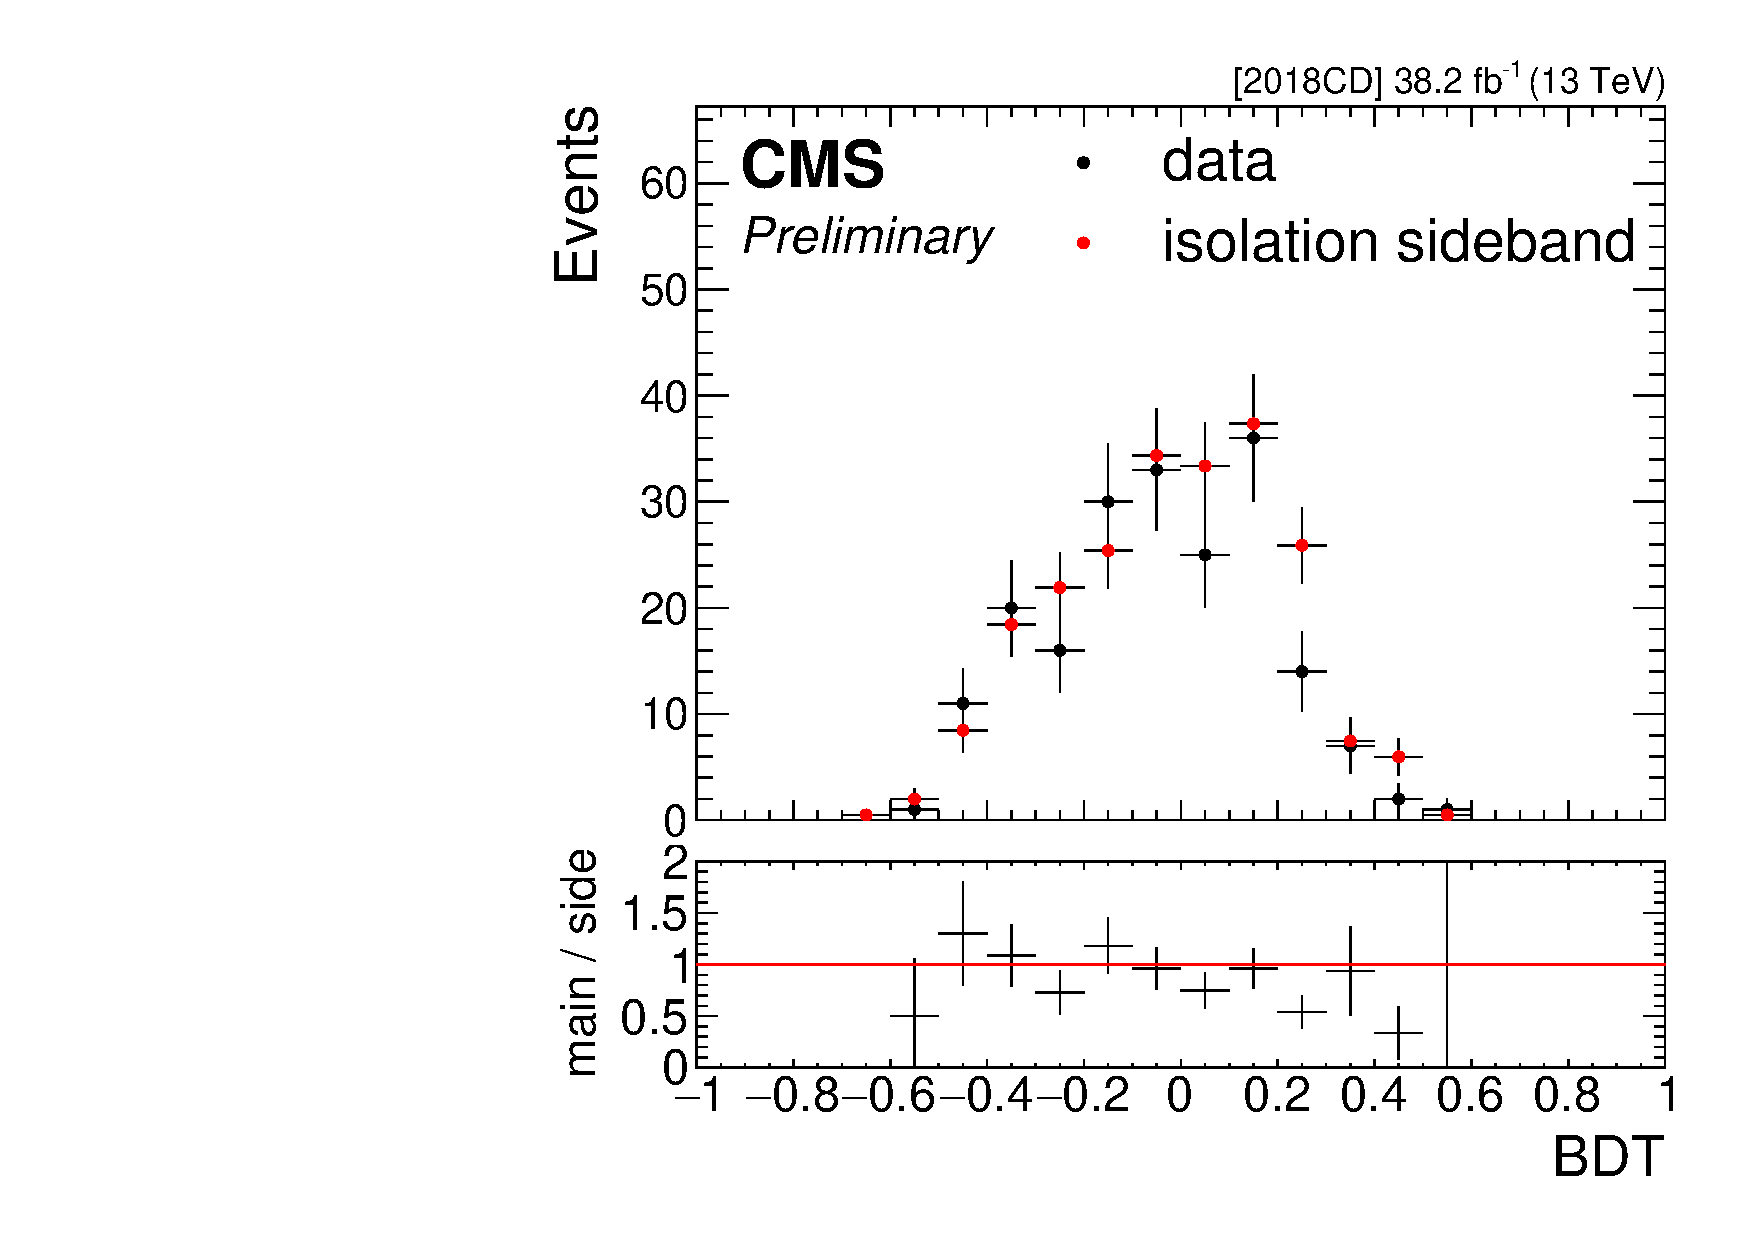
\includegraphics[width=0.48\linewidth]{plots/dilepton_muons_data_isocr_no_retag_CorrJetNoMultIso10_06_invmass_same_sign_2018CD/none_dilepBDTCorrJetNoMultIso10Dr0.6.pdf} \,
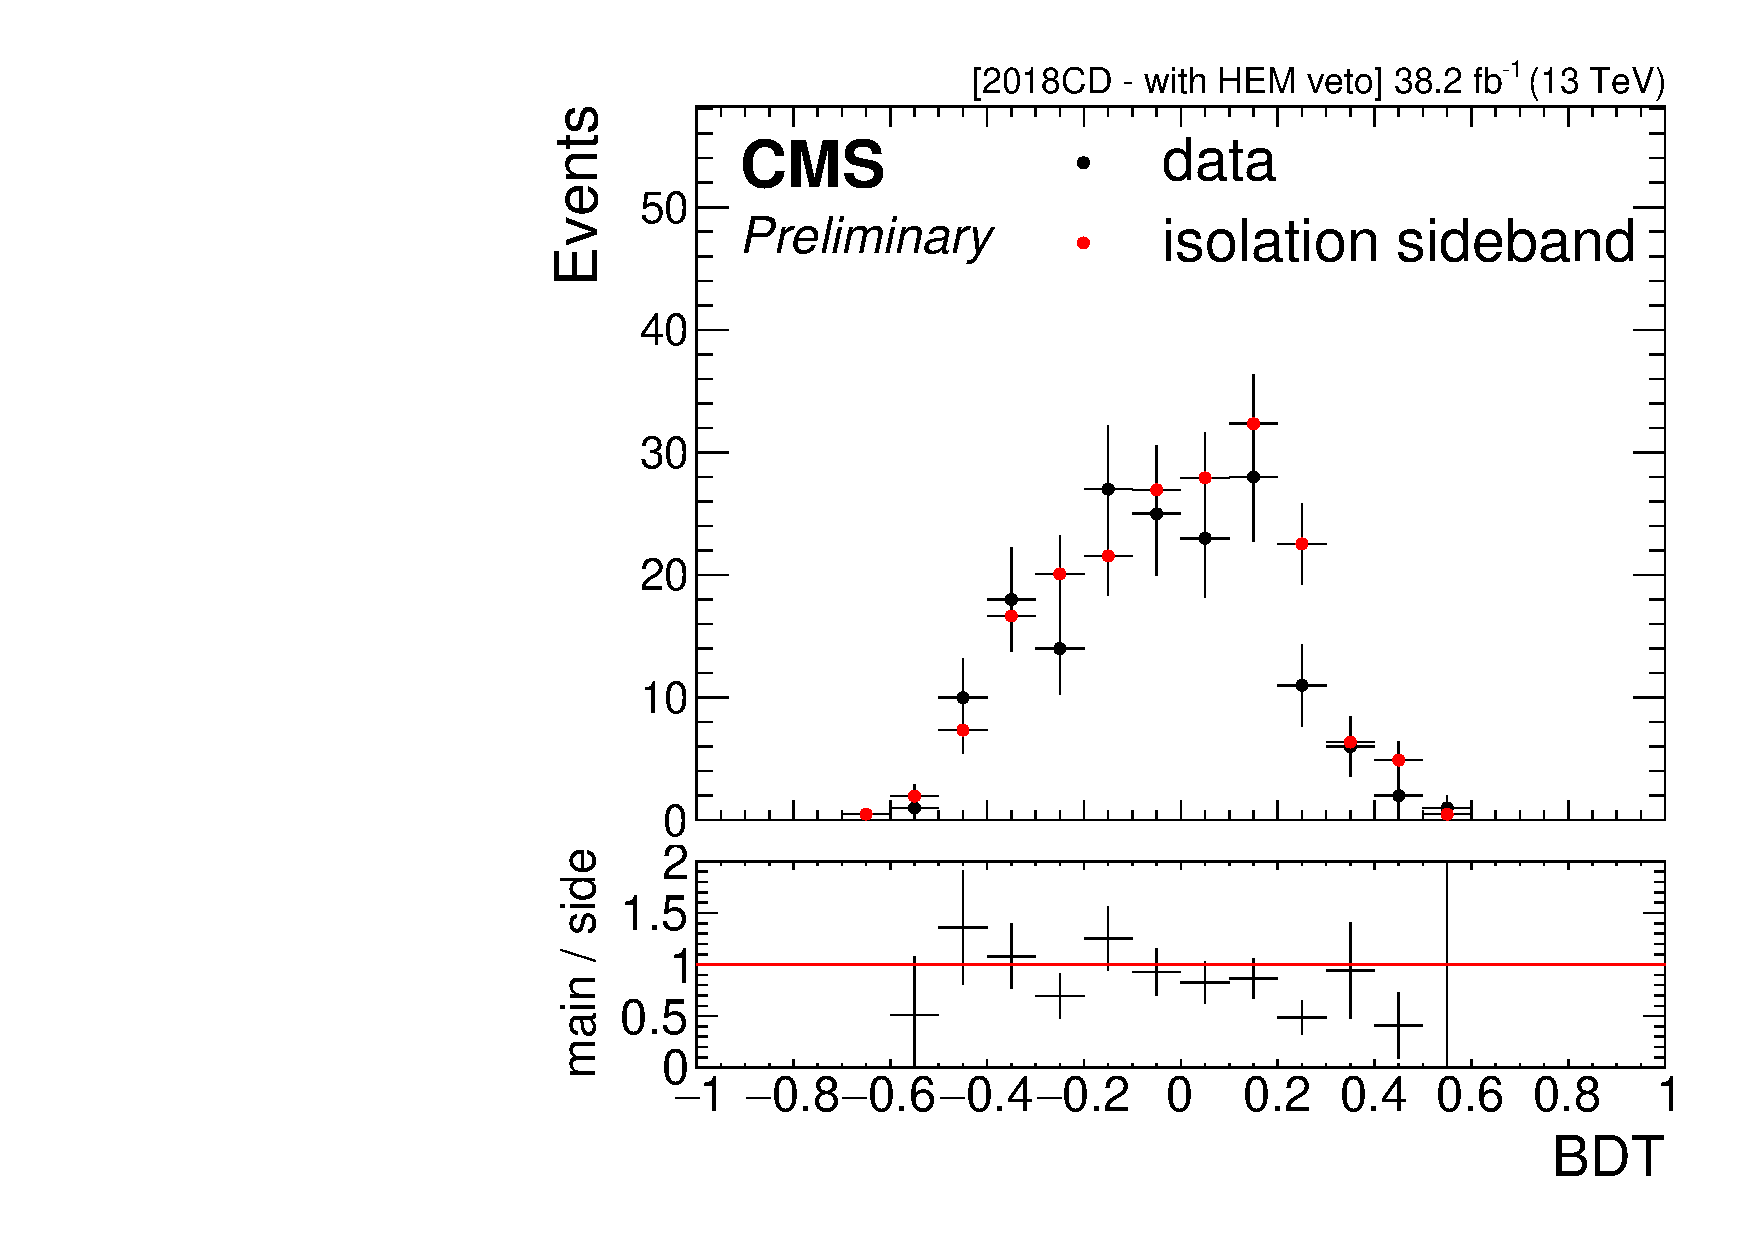
\includegraphics[width=0.48\linewidth]{plots/dilepton_muons_data_isocr_no_retag_CorrJetNoMultIso10_06_invmass_same_sign_2018CD_hem_veto/hem_ejm_dilepBDTCorrJetNoMultIso10Dr0.6.pdf} \\

\caption[Data same sign control validation plots]{Data same sign control validation plots. Black dots show same sign data in the main band, while red dots show same sign data in the isolation side band, normalized in the $\text{BDT}<0$ region. Ratio panel shows the ratio between them. Going line by line from left to right, the corresponding plots are shown: 2017 data taking period, 2017F data taking period, 2017F data taking period with prefire weights, 2018A data taking period (pre HEM), 2018CD data taking period (post HEM), 2018CD data taking period with HEM veto (post HEM).}
\label{fig:same-sign-validation-plots}
\end{figure}